\documentclass[a4paper,12pt]{article}
\usepackage{graphicx} 
\usepackage{hyperref}
\usepackage{float}
\usepackage{booktabs}
\usepackage{longtable}



% \begin{figure}[H]
%     \centering
%     \includegraphics[width=0.7\textwidth]{filename.png}
%     \caption{Your figure caption here.}
%     \label{fig:yourlabel}
% \end{figure}

\begin{document}

\title{Assignment 3 - Data Science\\
Brazillian e-commerce Analysis}
\author{Mohammad Hossein Basouli}
\date{\today}
\maketitle

\begin{center}
    \textit{\section*{Abstract}}
    \textit{In this analysis we will delve into the underlying relationships between different entities in a Brazilian e-commerce company and extract insights that help us in improving the sales in the company, 
    and understanding of the customer behaviors better. Some key insights, obtained from this analysis are as follows: We have figured out that there exists two different clusters of customers in terms of spendings, 
    one with very high and one with very low spendings - Also we can now say that the customers that buy expensive products, 
    tend to buy products that are heavy as well as having high volume - etc.}
\end{center}

% ---------------------------------------------------------------------------------------------------------------------------------------------------------------------------------------------------------------------- %

\section{Introduction}

\subsection{Background:} The analysis focuses on understanding customer behavior using data from a Brazilian e-commerce company. The process begins by setting clear objectives, 
followed by \textbf{Feature Engineering} to refine the dataset in the sections \textbf{Objectives} and \textbf{Feature Engineering}. Various clustering models are then applied to group, customers, with similar behaviors. 
These models are evaluated in the section \textbf{Models}, and the most effective one is used to analyze and interpret the behavioral patterns of different customer clusters, in the \textbf{Conclusion \& Decission Making}.

\subsection{Objectives:} 
\begin{enumerate}
    \item First, start off by cleaning the dataset; including handling inconsistency issues, missing values, etc.
    \item Utilizing our knowledge for Feature Engineering; provide justification for adding, keeping and removing features to the dataset.  
    \item Create a descriptive profile for each customer, by aggregation of information across the dataset, that can help in identifying the customer behaviors.
    \item Then develop different clustering methods to identify similar behaviors in the customers and divide them into several clusters.
    \item Evaluate the methods and see whether the customers are grouped into the correct clusters or not.
    \item Analyse the information, gained from the best clustering and gain insights from that.
\end{enumerate}

% ---------------------------------------------------------------------------------------------------------------------------------------------------------------------------------------------------------------------- %

\section{Feature Engineering:}
(In this section, whenever we talk say statistics, we mean \textit{min}, \textit{max}, \textit{mean}, \textit{total\_sum})
\begin{enumerate}
    \item Adding \textbf{proportion of each payment type}, used, by each customer; This will help to cluster customers, based on the \textit{Payment Type} that they prefer usually.
    \item Adding features that capture details of the payments that have taken place by each customer; such as about \textbf{payment\_value}, \textbf{payment\_installments}. These will help in identify patterns in purchase behaviors.
    \item Adding statistics about \textbf{product\_volume}, \textbf{product\_weight} and \textbf{\# of distinct products} bought by the customer. This gives information about the type of the products that customer tend to buy.
    \item Adding statistics about \textbf{review\_score}. This will tells us, how each user behaves in terms of giving review scores.
    \item Adding \textbf{\# of distinct sellers} that the customers have bought something from. 
\end{enumerate}

% ---------------------------------------------------------------------------------------------------------------------------------------------------------------------------------------------------------------------- %

\section{Models}

\subsection{K-means with PCA}
We first apply PCA (by maintaining 95 percent of the total variance in the data) on the dataset and then use it's components to fit a K-means to the dataset.  

\subsubsection{Hyper Parameter Tuning:}
\begin{figure}[H]
    \centering
    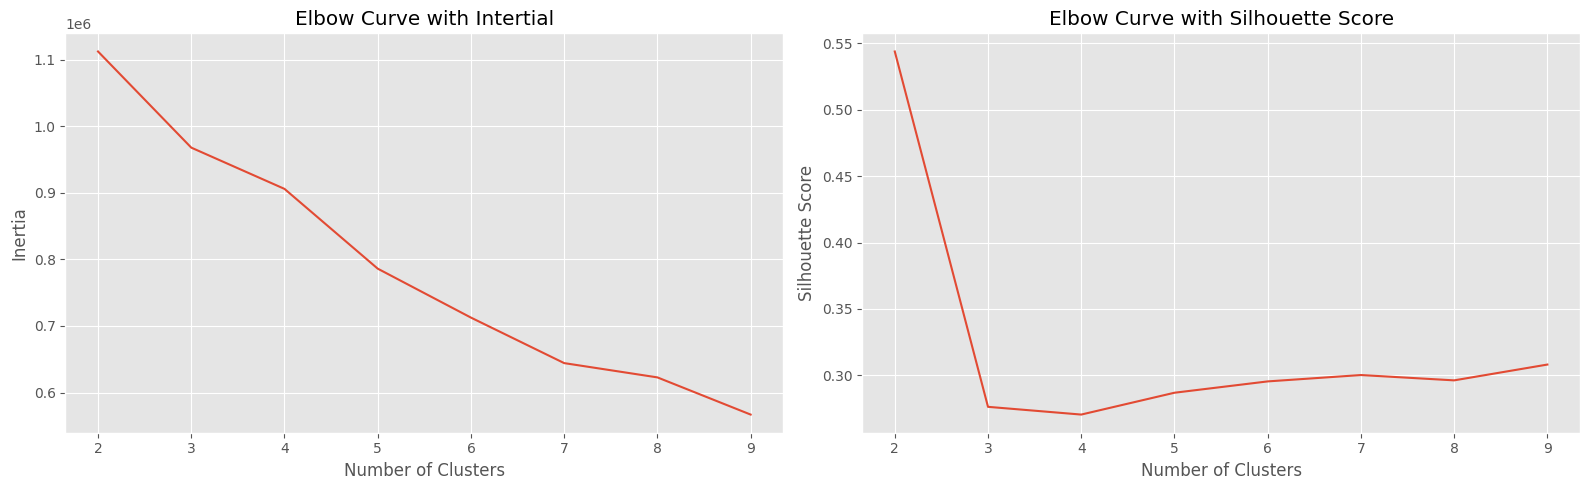
\includegraphics[width=1\textwidth]{./images/elbow_kmeans_pca.png}
    \caption{Elbow curve for K-means with PCA. The Elbow (for \textit{silhouette score}) reaches it's maximum at 2 clusters which has a \textit{silhouette score} around 0.55. 
    Thus we choose 2, as the number of clusters to be used for our K-means, which uses PCA for space transformation.}
    \label{fig:fig_1}
\end{figure}

\newpage

\subsubsection{Cluster Overlays on PCA:}
By looking at the Figures~\ref{fig:fig_2}, \ref{fig:fig_3}, we can see that the clusters are not separated very clearly and this might result, if we pick this model. 
This could be due to low quality features or an incorrect transformation of the feature space. \\ 

\noindent\textbf{3D Graph}
\begin{figure}[H]
    \centering
    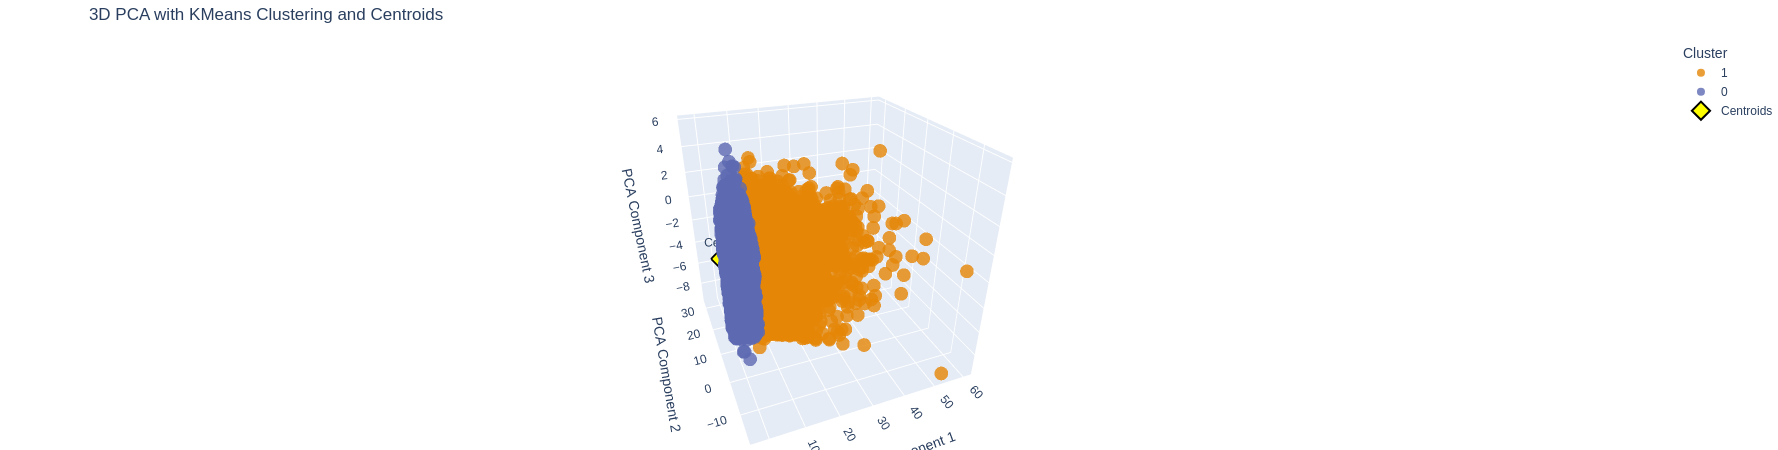
\includegraphics[width=1\textwidth]{./images/3d_pca_kmeans.png}
    \caption{3D cluster overlays on PCA. The figure shows that the clusters aren't separated well. This could be due to low quality of our features or inappropriate transformation of the feature space.}
    \label{fig:fig_2}
\end{figure}

\noindent\textbf{2D Graph}
\begin{figure}[H]
    \centering
    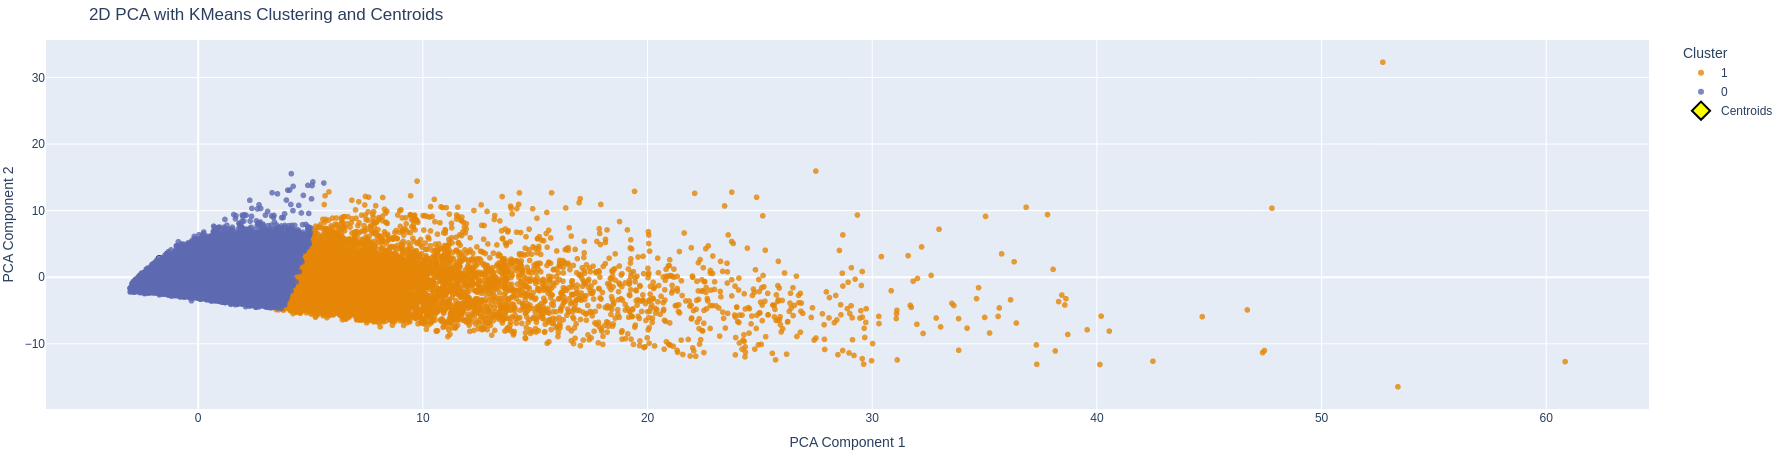
\includegraphics[width=1\textwidth]{./images/2d_pca_kmeans.png}
    \caption{2D cluster overlays on PCA. The figure shows the same thing as Figure~\ref{fig:fig_2}; that clusters aren't separated well.}
    \label{fig:fig_3}
\end{figure}

\subsubsection{Evaluation:}
Although as we saw in the Figure~\ref{fig:fig_1}, that the \textit{silhouette score} is really good (0.55) for this model, we guess that it wouldn't work very well, because it has failed to separate the customers into different clusters (Figures~\ref{fig:fig_2}, \ref{fig:fig_3}).


\subsection{K-means with t-SNE}
We first apply t-SNE (with 3 components) on the dataset to transfor the feature space to an space where we can possibly separate out the customers by some clusters. Then we use the transfored spaced to fit K-means on.  

\subsubsection{Hyper Parameter Tuning:}
\begin{figure}[H]
    \centering
    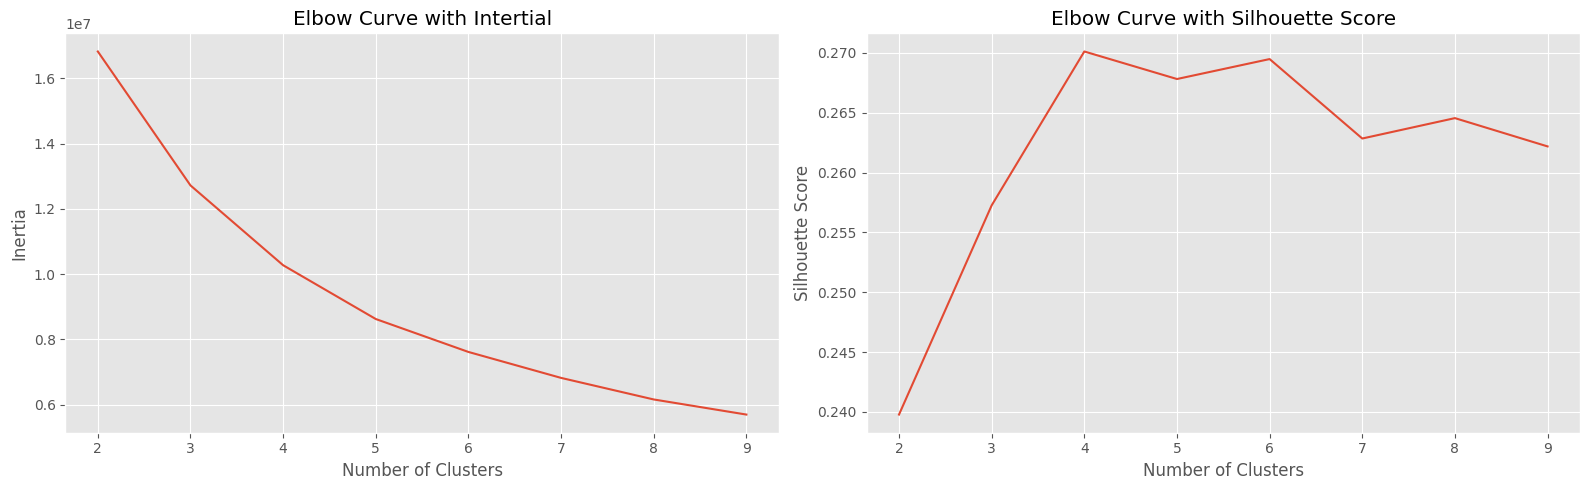
\includegraphics[width=1\textwidth]{./images/elbow_kmeans_tsne.png}
    \caption{Elbow curve for K-means with t-SNE. This curve is somehow controversy to Figure~\ref{fig:fig_1}, 
    since the optimal \textit{silhouette score} is reached at 4 clusters which had a very bad score in the previous Figures. Thus we select 4 as the number of clusters for our K-means model.}
    \label{fig:fig_4}
\end{figure}

\subsubsection{Cluster Overlays on t-SNE:}
Looking at the Figures~\ref{fig:fig_5} and \ref{fig:fig_6}, we find out, that the K-means with t-SNE transformation works so much better than the previous model (K-means with PCA transformation). \\

\newpage

\noindent\textbf{3D Graph}
\begin{figure}[H]
    \centering
    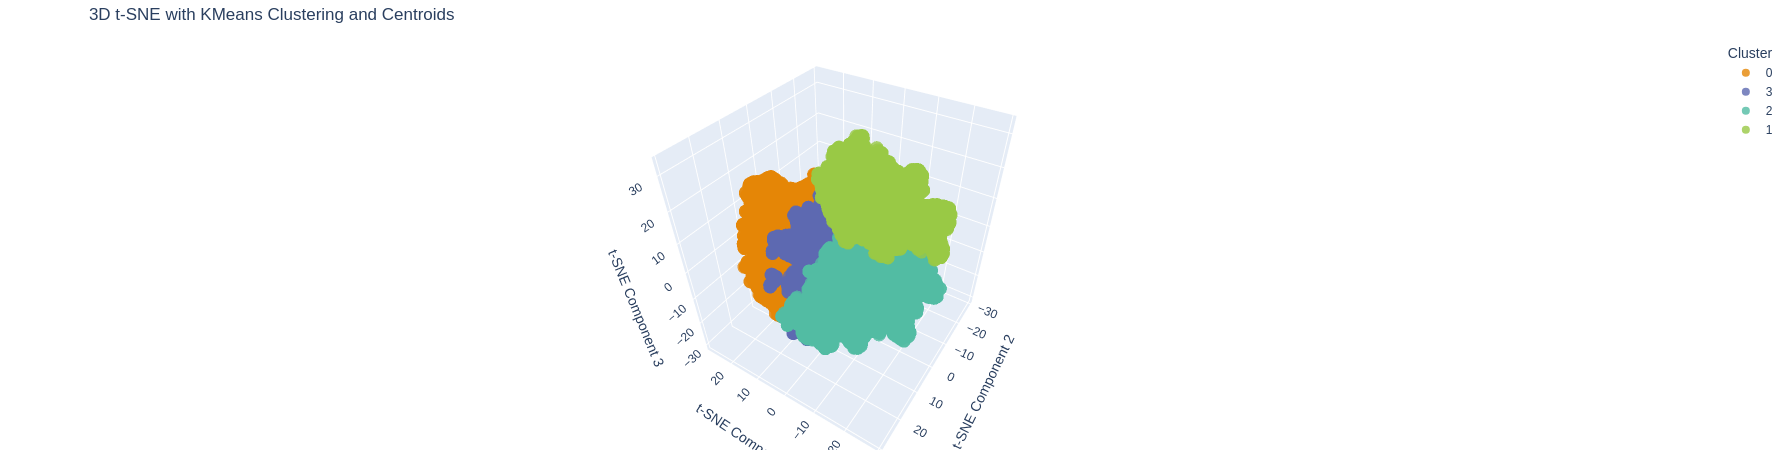
\includegraphics[width=1\textwidth]{./images/3d_tsne_kmeans.png}
    \caption{3D cluster overlays on t-SNE. This figure shows that, the K-means with t-SNE transformation seem to do a better job than the K-means with PCA transformation, since the clusters are separated better.}
    \label{fig:fig_5}
\end{figure}


\noindent\textbf{2D Graph}
\begin{figure}[H]
    \centering
    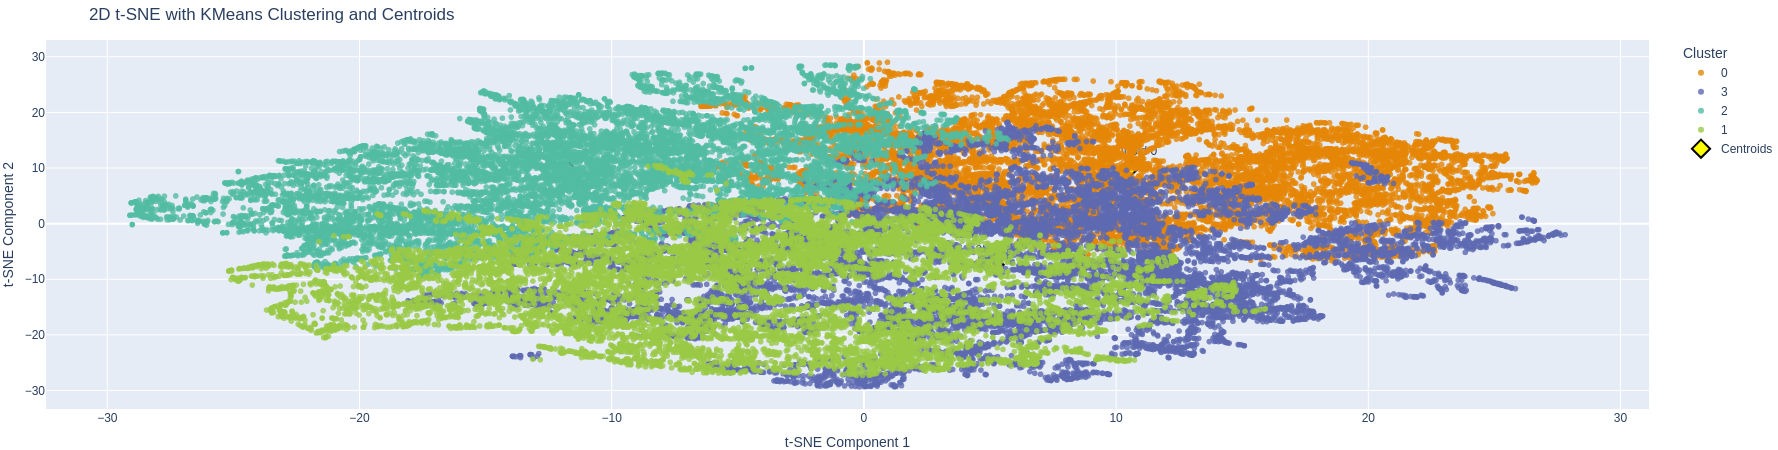
\includegraphics[width=1\textwidth]{./images/2d_tsne_kmeans.png}
    \caption{2D cluster overlays on t-SNE.}
    \label{fig:fig_6}
\end{figure}

\subsubsection{Evaluation:}
As we can see in Figure~\ref{fig:fig_4}, the \textit{silhouette score} for this model is decent (0.27). 
Also we can saw in \textbf{Cluster Overlays on t-SNE} subsection, we can say that it performs a good clustering on our data.



\subsection{DBSCAN with t-SNE}
We will first apply t-SNE (with 3 components) transformation on the dataset (since it seemed to be able to transform the feature space to an space where we can separate different group of customers), then apply DBSCAN.

\subsubsection{Hyper Parameter Tuning:}
By looking at the Figure~\ref{fig:fig_7}, we figure out that 1 might be an appropriate number of the \textbf{epsilon}, as the hyper parameter of our DBSCAN model. 
Also we set the minimum number of neighbors for a datapoint to be a core point in DBSCAN to be 2 * number of t-SNE components which is 3.

\begin{figure}[H]
    \centering
    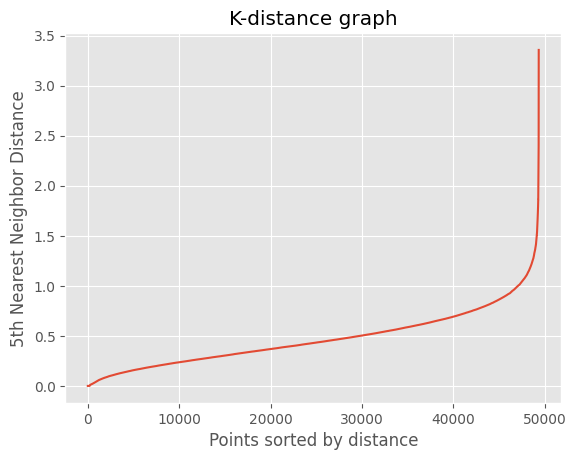
\includegraphics[width=1\textwidth]{./images/parameter_tuning_dbscan.png}
    \caption{Plot distances for different data points from their 5-th nearest neighbor. This plots tells us at most of the points have a distance around 0 to up to around 1, 
    thus we could use 1 as the epsilin hyper parameter of our DBSCAN model.}
    \label{fig:fig_7}
\end{figure}

\subsubsection{Cluster Overlays on t-SNE:}
By looking at the Figures~\ref{fig:fig_8} and \ref{fig:fig_9}, we figure out that our DBSCAN model works really bad, since it clusters each few points as a separate cluster.

\noindent\textbf{3D Graph}
\begin{figure}[H]
    \centering
    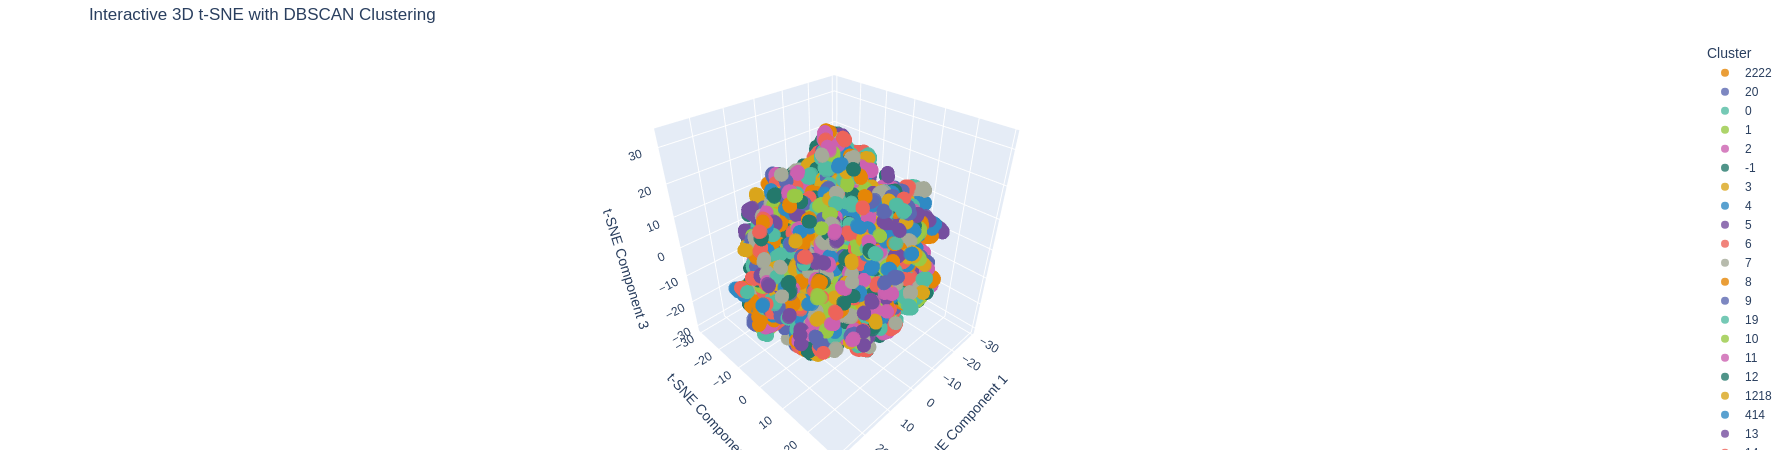
\includegraphics[width=1\textwidth]{./images/3d_tsne_dbscan.png}
    \caption{3D cluster overlays on t-SNE. The clustering is terrible! it takes each few points as a separate cluster.}
    \label{fig:fig_8}
\end{figure}

\noindent\textbf{2D Graph}
\begin{figure}[H]
    \centering
    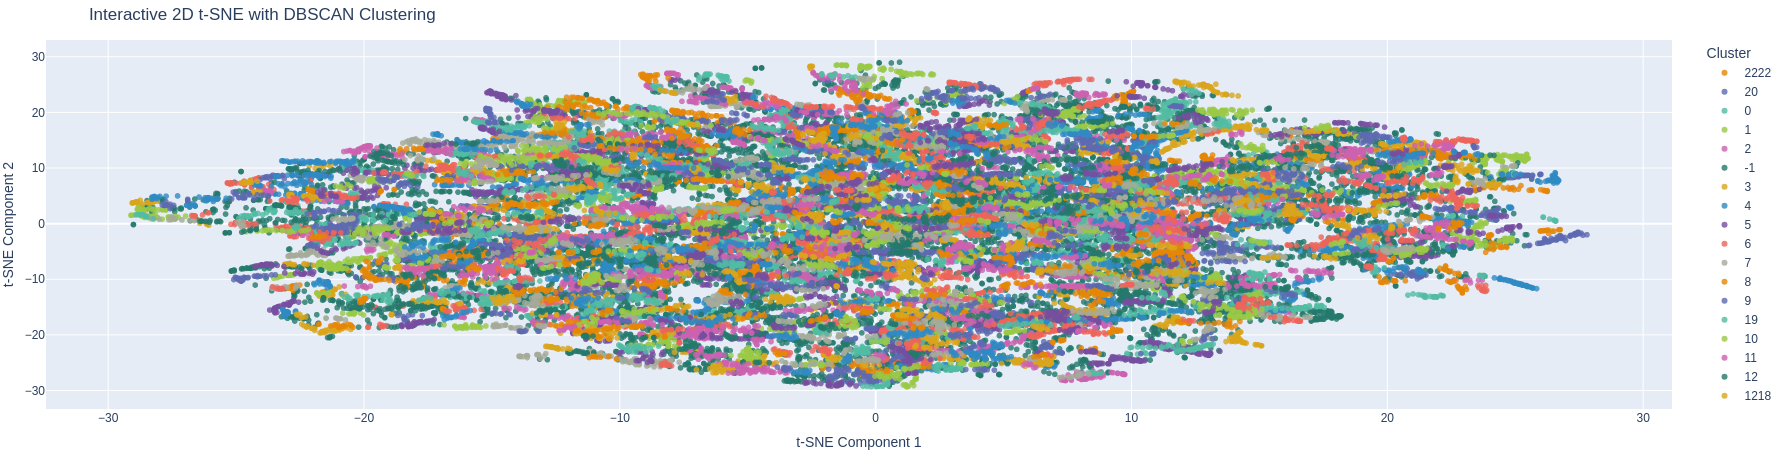
\includegraphics[width=1\textwidth]{./images/2d_tsne_dbscan.png}
    \caption{2D cluster overlays on t-SNE.}
    \label{fig:fig_9}
\end{figure}

\subsubsection{Evaluation:}
Although we get a really good \textit{silhouette score} for this model, this model is not good by any means, since it clusters each few points as a separate cluster.

\subsection{Conclusion on The Methodologies:}
As we saw in this section, the K-means model with t-SNE transformation, works the best, since it gets a moderate \textit{silhouette score}, and also as we can see from \textbf{Cluster Overlays on t-SNE}, this model causes the best separation between the clusters. Thus we choose this model for our analysis.

% ---------------------------------------------------------------------------------------------------------------------------------------------------------------------------------------------------------------------- %

\section{Conclusion \& Decission Making:}

\subsection*{Statistics For The Clusters:}

\begin{longtable}{lrrrrrrrr}
\caption{Summary Statistics by Cluster} \\
\toprule
\multicolumn{9}{l}{\textbf{Payment by Boleto Proportion}} \\
\midrule
Cluster & Count & Mean & Std & Min & 25\% & 50\% & 75\% & Max \\
\midrule
0 & 12118 & 0.0086 & 0.0922 & 0.0 & 0.0 & 0.0 & 0.0 & 1.0 \\
1 & 12395 & 0.3271 & 0.4692 & 0.0 & 0.0 & 0.0 & 1.0 & 1.0 \\
2 & 11507 & 0.0000 & 0.0000 & 0.0 & 0.0 & 0.0 & 0.0 & 0.0 \\
3 & 13312 & 0.4259 & 0.4945 & 0.0 & 0.0 & 0.0 & 1.0 & 1.0 \\
\midrule
\multicolumn{9}{l}{\textbf{Payment by Credit Card Proportion}} \\
\midrule
0 & 12118 & 0.9878 & 0.1069 & 0.0 & 1.0 & 1.0 & 1.0 & 1.0 \\
1 & 12395 & 0.6685 & 0.4684 & 0.0 & 0.0 & 1.0 & 1.0 & 1.0 \\
2 & 11507 & 0.9824 & 0.1253 & 0.0 & 1.0 & 1.0 & 1.0 & 1.0 \\
3 & 13312 & 0.4365 & 0.4802 & 0.0 & 0.0 & 0.0 & 1.0 & 1.0 \\
\midrule
\multicolumn{9}{l}{\textbf{Average Payment Value}} \\
\midrule
0 & 12118 & 273.79 & 351.52 & 7.68 & 104.19 & 168.36 & 293.44 & 7274.88 \\
1 & 12395 & 94.09 & 61.56 & 9.02 & 49.82 & 76.98 & 122.83 & 573.18 \\
2 & 11507 & 98.71 & 70.90 & 7.24 & 47.71 & 77.57 & 129.21 & 629.27 \\
3 & 13312 & 161.68 & 162.48 & 1.74 & 63.03 & 114.03 & 198.76 & 2234.66 \\
\midrule
\multicolumn{9}{l}{\textbf{Average Payment Installments}} \\
\midrule
0 & 12118 & 6.23 & 2.84 & 1.0 & 4.0 & 6.0 & 8.0 & 24.0 \\
1 & 12395 & 1.27 & 0.50 & 0.0 & 1.0 & 1.0 & 2.0 & 6.0 \\
2 & 11507 & 2.19 & 1.28 & 1.0 & 1.0 & 2.0 & 3.0 & 8.0 \\
3 & 13312 & 2.05 & 2.06 & 1.0 & 1.0 & 1.0 & 2.0 & 24.0 \\
\midrule
\multicolumn{9}{l}{\textbf{Average Product Volume}} \\
\midrule
0 & 12118 & 21483.29 & 31508.40 & 352.0 & 3960.0 & 10240.0 & 27000.0 & 296208.0 \\
1 & 12395 & 9750.52 & 11152.06 & 168.0 & 2520.0 & 5040.0 & 13200.0 & 87500.0 \\
2 & 11507 & 9341.54 & 11348.86 & 352.0 & 2378.0 & 4732.0 & 12000.0 & 101528.0 \\
3 & 13312 & 19993.91 & 28253.57 & 352.0 & 2964.0 & 8000.0 & 23625.0 & 262080.0 \\
\midrule
\multicolumn{9}{l}{\textbf{Average Product Weight}} \\
\midrule
0 & 12118 & 3163.41 & 4879.28 & 0.0 & 460.0 & 1200.0 & 3571.5 & 30000.0 \\
1 & 12395 & 1079.49 & 1583.46 & 2.0 & 250.0 & 533.0 & 1250.0 & 16283.0 \\
2 & 11507 & 1112.53 & 1690.64 & 2.0 & 233.0 & 500.0 & 1200.0 & 13350.0 \\
3 & 13312 & 3038.85 & 4812.18 & 50.0 & 300.0 & 850.0 & 3000.0 & 40425.0 \\
\midrule
\multicolumn{9}{l}{\textbf{\# of Distinct Bought Products}} \\
\midrule
0 & 12118 & 1.057 & 0.280 & 1.0 & 1.0 & 1.0 & 1.0 & 7.0 \\
1 & 12395 & 1.000 & 0.000 & 1.0 & 1.0 & 1.0 & 1.0 & 1.0 \\
2 & 11507 & 1.000 & 0.000 & 1.0 & 1.0 & 1.0 & 1.0 & 1.0 \\
3 & 13312 & 1.090 & 0.337 & 1.0 & 1.0 & 1.0 & 1.0 & 6.0 \\
\midrule
\multicolumn{9}{l}{\textbf{Average Freight Value}} \\
\midrule
0 & 12118 & 26.40 & 24.32 & 0.0 & 15.11 & 18.74 & 27.55 & 409.68 \\
1 & 12395 & 15.68 & 4.87 & 0.0 & 12.79 & 15.23 & 18.23 & 56.61 \\
2 & 11507 & 15.97 & 7.80 & 0.0 & 10.95 & 15.10 & 18.23 & 68.40 \\
3 & 13312 & 22.45 & 16.39 & 0.0 & 14.10 & 17.60 & 24.09 & 209.63 \\
\midrule
\multicolumn{9}{l}{\textbf{Average Review Score}} \\
\midrule
0 & 12118 & 4.51 & 1.02 & 1.0 & 4.11 & 5.0 & 5.0 & 5.0 \\
1 & 12395 & 5.00 & 0.04 & 4.0 & 5.0 & 5.0 & 5.0 & 5.0 \\
2 & 11507 & 4.06 & 0.78 & 2.0 & 4.0 & 4.0 & 5.0 & 5.0 \\
3 & 13312 & 2.93 & 1.66 & 1.0 & 1.0 & 3.0 & 5.0 & 5.0 \\
\midrule
\multicolumn{9}{l}{\textbf{\# of Distinct Sellers}} \\
\midrule
0 & 12118 & 1.05 & 0.23 & 1.0 & 1.0 & 1.0 & 1.0 & 5.0 \\
1 & 12395 & 1.00 & 0.00 & 1.0 & 1.0 & 1.0 & 1.0 & 1.0 \\
2 & 11507 & 1.00 & 0.00 & 1.0 & 1.0 & 1.0 & 1.0 & 1.0 \\
3 & 13312 & 1.01 & 0.08 & 1.0 & 1.0 & 1.0 & 1.0 & 2.0 \\
\bottomrule
\end{longtable}

\subsection{Cluster Profiling:}
We will list the key statistics for of each of the clusters below:
\begin{itemize}
    \item Cluster 0 and 2:
    \begin{enumerate}
        \item These two groups have a high spending.
        \item They pay a great amount of money for freight.
        \item They buy products with high volumes.
        \item They usually buy heavy products.
    \end{enumerate}
    \item Cluster 1 and 3:
    \begin{enumerate}
        \item These two groups have a low spending.
        \item They pay a low amount of money for freight.
        \item They buy products with low volumes.
        \item They usually buy light products.
    \end{enumerate}
    \item Cluster 0: Have the lowest review score.
    \item Cluster 1: Have the highest review score.
    \item Cluster 2: Have decent review score. 
    \item Cluster 3: Have a decent review score.
\end{itemize}

\subsection{Cluster Labeling:}
\begin{itemize}
    \item Cluster 0: \textbf{VIP complainers}.
    \item Cluster 1: \textbf{Happy Campers}.
    \item Cluster 2: \textbf{Steady Royals}.
    \item Cluster 3: \textbf{Budget Buddies}.
\end{itemize}

\subsection*{Decission Making:}
\begin{itemize}
    \item \textbf{Cluster 0}
    \begin{enumerate}
        \item Improve customer service and post-purchase experience (e.g., faster response times, better packaging, easier returns) to address the low review scores despite high spending.
        \item Introduce loyalty rewards or discounts on freight costs to retain these high-value customers and potentially improve satisfaction and reviews.
    \end{enumerate}

    \item \textbf{Cluster 1}
    \begin{enumerate}
        \item Upsell or cross-sell heavier or higher-volume products by leveraging the high satisfaction scores and trust these customers already have.
        \item Introduce premium product options or bundles to gradually increase spending while maintaining their positive experience.
    \end{enumerate}

    \item \textbf{Cluster 2}
    \begin{enumerate}
        \item Highlight and promote their positive experiences through reviews or testimonials to reinforce purchasing behavior and encourage higher engagement.
        \item Offer freight discounts or subscription-based shipping services to reward their high freight spending and encourage loyalty.
    \end{enumerate}

    \item \textbf{Cluster 3}
    \begin{enumerate}
        \item Provide incentives (e.g., small discounts, free samples) for larger purchases to increase volume without compromising satisfaction.
        \item Conduct targeted marketing based on their decent satisfaction levels to push mid-range or higher-margin products.
    \end{enumerate}
\end{itemize}








\end{document}